% Figura 1 de la postulación: arquitectura general del modelo de SAM-Cordillera.
% Tres bloques, uno por subpunto: severidad y peligro (5.1), despeje (5.2) y estados operacionales (5.3).
\documentclass[border=4pt]{standalone}
% Preámbulo común de las figuras 1 a 4 de la postulación (se carga con \input en cada figura).
% Los cortes y umbrales vienen de umbrales_calibrados.tex (lo escribe figuras_postulacion.py).
\usepackage{fontspec}
\setmainfont{Cambria}
\usepackage[table]{xcolor}
\usepackage{array,booktabs}
\usepackage{tikz}
\usetikzlibrary{arrows.meta,positioning,calc,fit,backgrounds,decorations.pathreplacing}
\definecolor{fondo}{HTML}{F2F1EC}
\definecolor{txt2}{HTML}{52514E}
% estados, ordenados por magnitud: E3 despeje < E4 tormenta < E5 peligro
\definecolor{cE0}{HTML}{D9D8D2}\definecolor{cE1}{HTML}{1BAF7A}\definecolor{cE2}{HTML}{EDA100}
\definecolor{cE3}{HTML}{2A78D6}\definecolor{cE4}{HTML}{E34948}\definecolor{cE5}{HTML}{4A3AA7}
\definecolor{cSV}{HTML}{2A78D6}\definecolor{cH}{HTML}{EB6834}\definecolor{cN}{HTML}{52514E}
% Generado por figuras_postulacion.py desde salidas/sistema/parametros.json. No editar a mano.
\newcommand{\cortesS}{\textbf{0{,}5} & 5 & \textbf{12{,}5} & 20 & \textbf{25}}
\newcommand{\cortesF}{0{,}05 & 0{,}25 & 0{,}50 & 0{,}75 & 0{,}95}
\newcommand{\cortesr}{0{,}5 & 1 & 2 & 3 & 4}
\newcommand{\cortesdur}{1 & 6 & 12 & 18 & 23}
\newcommand{\cortesG}{10 & 15 & 20 & 25 & 30}
\newcommand{\cortesR}{\textbf{0{,}5} & 2{,}5 & 5 & \textbf{10} & 15}
\newcommand{\cortesHNS}{10 & 20 & 30 & 50 & 80}
\newcommand{\cortesRS}{10 & 20 & 40 & 60 & 100}
\newcommand{\pesoS}{0{,}45}
\newcommand{\pesoF}{0{,}15}
\newcommand{\pesor}{0{,}10}
\newcommand{\pesodur}{0{,}10}
\newcommand{\pesoG}{0{,}10}
\newcommand{\pesoR}{0{,}10}
\newcommand{\SVrest}{1}
\newcommand{\SVparc}{2{,}5}
\newcommand{\SVcierre}{3{,}5}
\newcommand{\Hrest}{3}
\newcommand{\Hparc}{4}
\newcommand{\Hcierre}{5}
\newcommand{\Nrest}{5}
\newcommand{\Nparc}{30}
\newcommand{\Ncierre}{50}
\newcommand{\cdesp}{6}
\newcommand{\expAlto}{1}
\newcommand{\expMedio}{0{,}5}
\newcommand{\hnSobrecarga}{30}

\newcolumntype{L}[1]{>{\raggedright\arraybackslash}p{#1}}
\newcolumntype{C}{>{\centering\arraybackslash}p{0.62cm}}
% encabezado de notas con degradado del color del índice
\newcommand{\notas}[1]{\cellcolor{#1!12}1 & \cellcolor{#1!28}2 & \cellcolor{#1!45}3 & \cellcolor{#1!65}\textcolor{white}{4} & \cellcolor{#1!85}\textcolor{white}{5}}
\tikzset{
  tit/.style={anchor=north west, font=\small\bfseries, inner sep=0pt},
  caja/.style={draw=#1, line width=0.9pt, rounded corners=3pt, align=center, minimum width=4.2cm, minimum height=1.05cm, fill=white},
  dato/.style={draw=txt2, dashed, rounded corners=3pt, align=center, minimum width=4.5cm, minimum height=0.85cm},
  est/.style={rounded corners=2pt, align=center, minimum width=1.98cm, minimum height=1.05cm, font=\scriptsize, text=white, inner sep=1pt},
  niv/.style={rounded corners=2pt, align=center, minimum width=2.45cm, minimum height=0.62cm, font=\scriptsize, inner sep=1pt},
  llave/.style={decorate, decoration={brace, amplitude=3pt}, draw=txt2},
  flecha/.style={-{Stealth[length=2mm]}, thick, draw=txt2},
  eti/.style={font=\scriptsize, color=txt2, align=center}}

\begin{document}
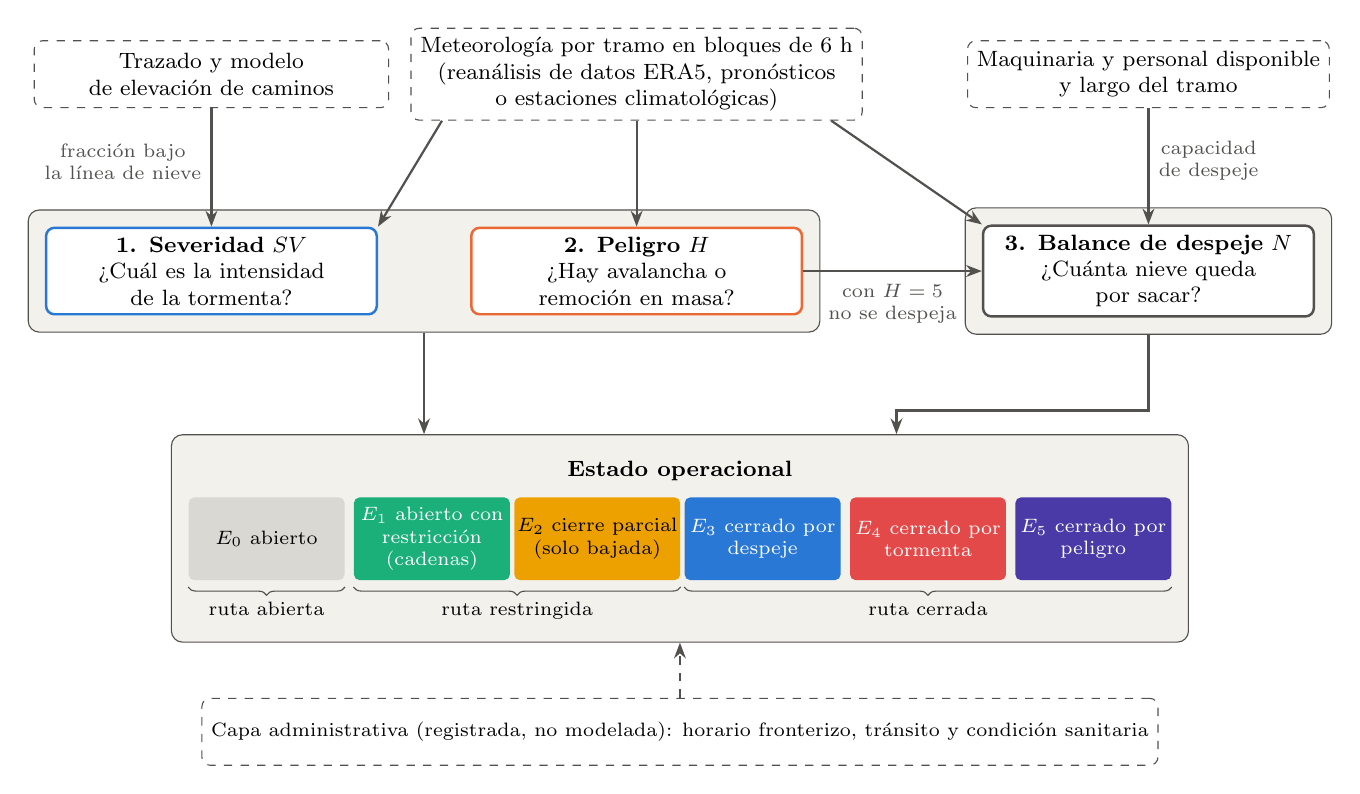
\begin{tikzpicture}[font=\footnotesize,
  bloque/.style={draw=txt2, rounded corners=4pt, fill=fondo, inner xsep=6pt, inner ysep=6pt}]
% entradas
\node[dato] (dem) at (2.3,-1.05) {Trazado y modelo\\de elevación de caminos};
\node[dato, minimum width=5.2cm] (era) at (7.7,-1.05) {Meteorología por tramo en bloques de 6 h\\(reanálisis de datos ERA5, pronósticos\\o estaciones climatológicas)};
\node[dato] (maq) at (14.2,-1.05) {Maquinaria y personal disponible\\y largo del tramo};
% índices
\node[caja=cSV] (sv) at (2.3,-3.55) {\textbf{1. Severidad} $SV$\\¿Cuál es la intensidad\\de la tormenta?};
\node[caja=cH] (h) at (7.7,-3.55) {\textbf{2. Peligro} $H$\\¿Hay avalancha o\\remoción en masa?};
\node[caja=cN] (n) at (14.2,-3.55) {\textbf{3. Balance de despeje} $N$\\¿Cuánta nieve queda\\por sacar?};
\begin{scope}[on background layer]
\node[bloque, fit=(sv)(h)] (b51) {};
\node[bloque, fit=(n)] (b52) {};
\end{scope}
\draw[flecha] (era) -- (h);
\draw[flecha] (era.south west) ++(0.4,0) -- (sv.north east);
\draw[flecha] (era.south east) ++(-0.4,0) -- (n.north west);
\draw[flecha] (dem) -- node[eti, left, pos=0.45]{fracción bajo\\la línea de nieve} (sv);
\draw[flecha] (maq) -- node[eti, right, pos=0.45]{capacidad\\de despeje} (n);
\draw[flecha] (h) -- node[eti, below=1pt]{con $H = \Hcierre$\\no se despeja} (n);
% estados operacionales, ordenados por magnitud
\foreach \e/\txt/\col/\x in {0/abierto/black/3.0,
                             1/abierto con\\restricción\\(cadenas)/white/5.1,
                             2/cierre parcial\\(solo bajada)/black/7.2,
                             3/cerrado por\\despeje/white/9.3,
                             4/cerrado por\\tormenta/white/11.4,
                             5/cerrado por\\peligro/white/13.5}
  \node[est, fill=cE\e, text=\col] (e\e) at (\x,-6.95) {\textbf{$E_\e$} \txt};
\node[font=\footnotesize\bfseries, anchor=south] (tite) at ($(e0.north)!0.5!(e5.north)+(0,0.08)$) {Estado operacional};
\draw[llave] ($(e0.south east)+(0,-0.08)$) -- node[below=2pt, font=\scriptsize] (g1) {ruta abierta} ($(e0.south west)+(0,-0.08)$);
\draw[llave] ($(e2.south east)+(0,-0.08)$) -- node[below=2pt, font=\scriptsize] {ruta restringida} ($(e1.south west)+(0,-0.08)$);
\draw[llave] ($(e5.south east)+(0,-0.08)$) -- node[below=2pt, font=\scriptsize] {ruta cerrada} ($(e3.south west)+(0,-0.08)$);
\begin{scope}[on background layer]
\node[bloque, fit=(e0)(e5)(tite)(g1)] (b53) {};
\end{scope}
% de los índices al estado
\coordinate (x51) at (5.0,0);
\coordinate (x52) at (11.0,0);
\draw[flecha] (b51.south -| x51) -- (b53.north -| x51);
\draw[flecha] (b52.south) |- ($(b53.north -| x52)+(0,0.3)$) -- (b53.north -| x52);
\node[dato, minimum width=9cm, font=\scriptsize, anchor=north] (adm) at ($(b53.south)+(0,-0.7)$) {Capa administrativa (registrada, no modelada): horario fronterizo, tránsito y condición sanitaria};
\draw[flecha, dashed] (adm.north) -- (b53.south);
\end{tikzpicture}
\end{document}
